\documentclass[../_main/handlingar.tex]{subfiles}

\begin{document}
\proposition{Uppdatering av medaljpolicyn}

Policyn för \emph{Sektionens medaljer och dess utdelning} är i det stora hela bra skriven men vi anser att avsnittet om utdelning är lite väl detaljstyrande och att några små omstruktureringar skulle göra policyn tydligare och mer lättläst. Till sist tycker vi att det vore bra om policyn kompletteras med bilder på medaljerna för att underlätta för de som ska dela ut dessa.

Med ovanstående som utgångspunkt yrkar styrelsen på

\begin{attsatser}
    \att flytta stycket om Styrelsemedalj och dess beskrivning från avsnittet E-sektionens förtjänstmedaljer till stycket E-sektionens Funktionärsmedaljer,
    \att direkt under avsnittet E-sektionens Funktionärsmedaljer lägga till “Sigillbevararen tillsammans med styrelsen avgör vem som gjort sig förtjänt av en funktionärsmedalj. Detta beslut baseras på om personen i fråga fullgjort sitt åtagande i enlighet med reglementet.”,
    \att direkt under avsnittet E-sektionens förtjänstmedaljer lägga till “Mottagare av följande medaljer utses av sigillbevararen tillsammans med styrelsen. Medaljerna ska utdelas på någon av Sektionens högtidligaste sammankomster som till exempel Nollegasquen eller vid Jubileum dit mottagaren av Krusidull-E:t ska bli inbjuden”,
    \att stryka stycket utdelning, samt
    \att lägga till bifogad bild på medaljerna med tillhörande bildtext “Sektionens medaljer. Från vänster: Funktionärsmedalj 1 år med tillägg för 3 samt 5 år, Styrelsemedalj, Bidragsmedalj, Utomstående Förtjänstmedalj samt Krusidull-E.”
\end{attsatser}

\vspace*{\baselineskip}

\begin{center}
    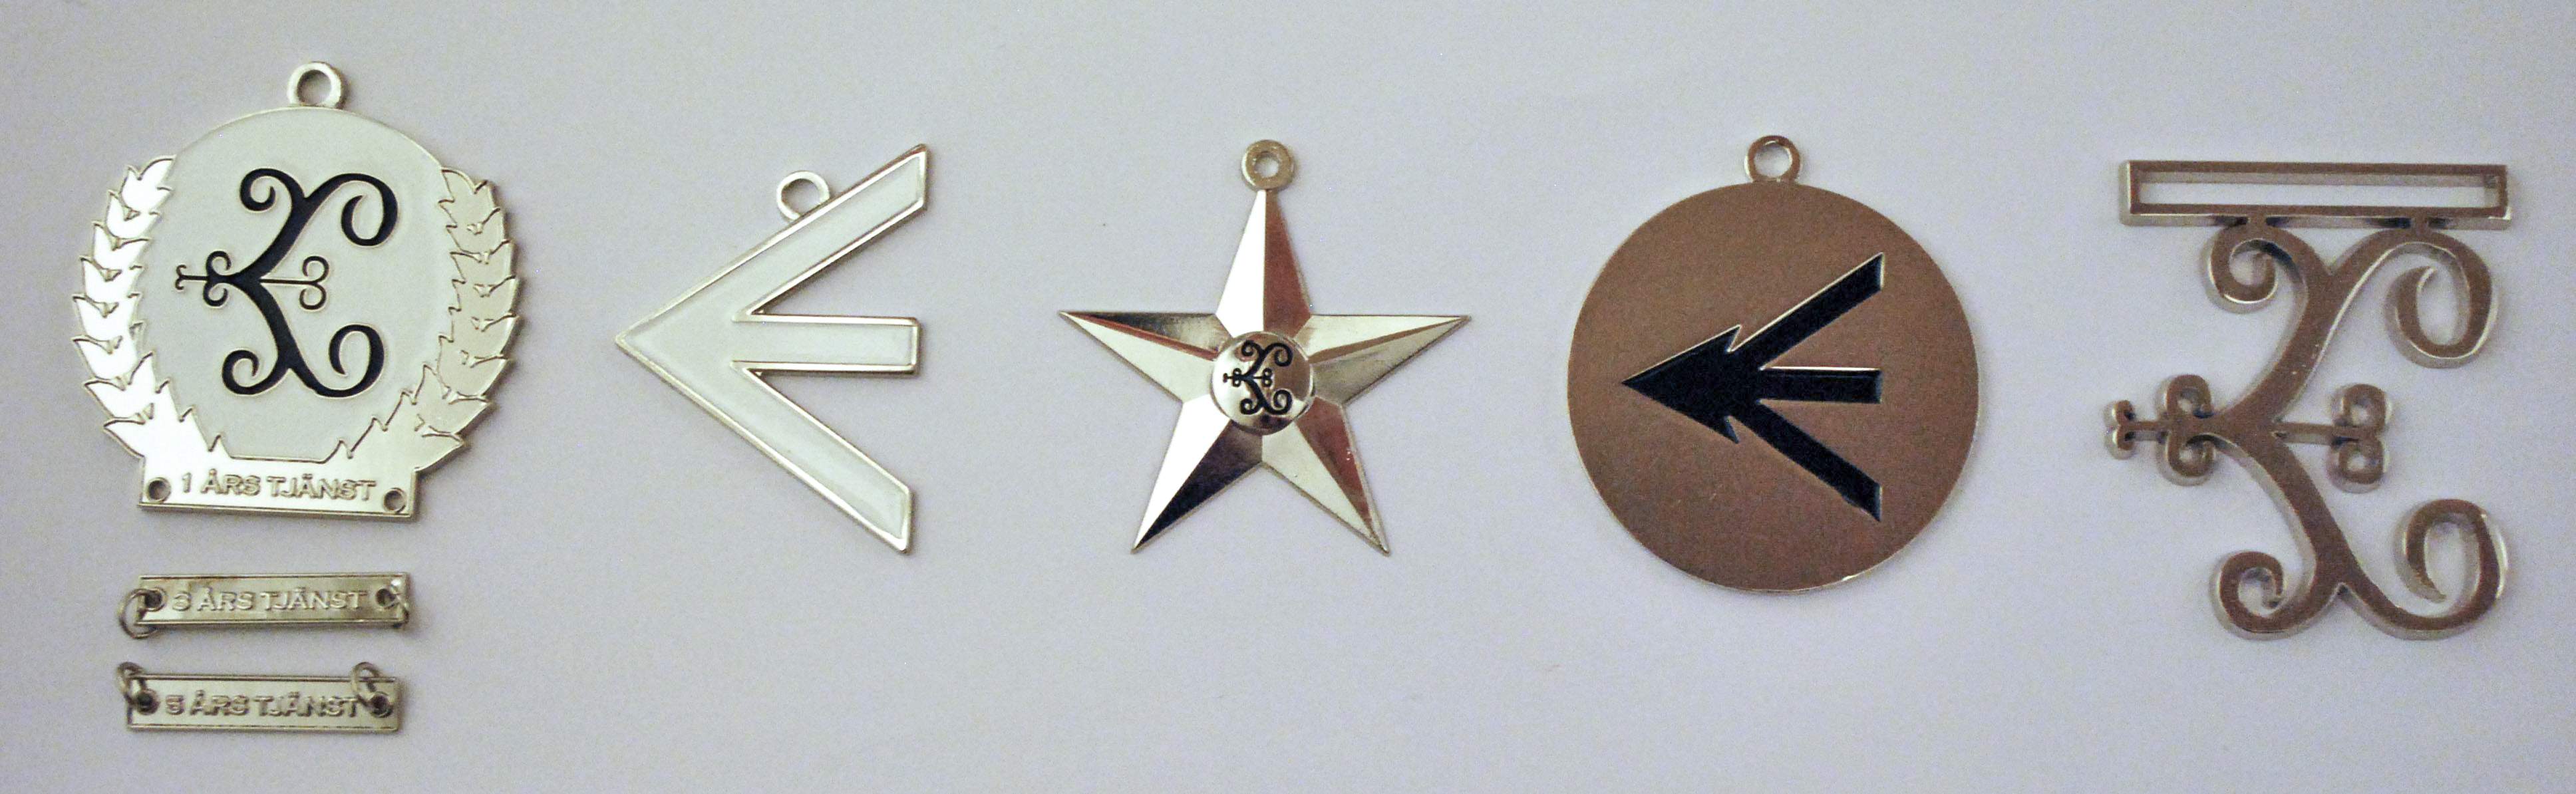
\includegraphics[width=0.8\textwidth]{medaljer.jpg}
\end{center}

\begin{signatures}{1}
    \ist
    \signature{\ordf}{Ordförande}
\end{signatures}

\end{document}
